\section{Theorie}
\label{sec:Theorie}
Zur Messung ionisierender Strahlung wird das Geiger-Müller-Zählrohr genutzt, an dessen Ausgang kann ein
Impulszähler angeschlossen und damit kann die Intensität gemessen werden.
Die Apparatur besteht aus einem Metallzylinder, dieser dient als Kathode, mit Radius $r_\mathrm{k}$ und
einem Anodendraht mit Radius $r_\mathrm{a}$, das Innere ist gefüllt mit einem Gasgemisch aus Argon und Ethylalkohol.
Beim Anlegen einer Spannung entsteht ein elektrisches Feld, damit wird die Bewegung der eingehenden Teilchen beeinflusst.
Die Teilchen weisen unterschiedliches Verhalten bei verschiendenen Spannungen auf, somit enstehen verschiedene Abschnitte, wie
in Abbildung \ref{fig:bereich} zu sehen.
\begin{figure}
  \centering
  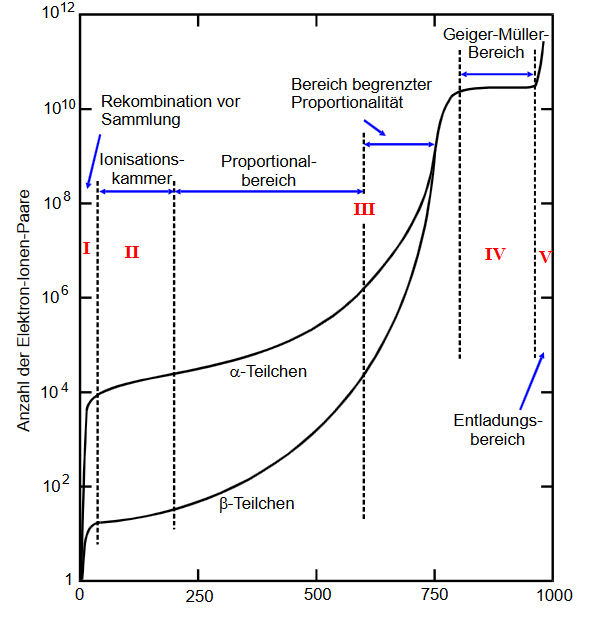
\includegraphics[width=0.5\textwidth]{bereiche.PNG}
  \caption{Verschiedene Zonen des Widerstandes.}
  \label{fig:bereich}
\end{figure}
Zone $I$ stellt die geringen Spannungen dar, dabei erreichen kaum Elektronen den Draht, zuvor rekombinieren die restlichen Elektronen.
